\section{Рассеяние частиц. Формула Резерфорда.}

% Нужно больше комментариев по ходу решения задач: объяснять что и откуда
% находится. Например, в первой задаче -- что такое E_1, E_2, E_внут и т.д.,
% а в 4.4 вообще ни одного слова

\begin{enumerate}
% 4.1 --------------
\item Исходя из томпсоновской модели атома, определить:
\begin{enumerate}
    \item радиус атома водорода, энергия ионизации которого 13,6~эВ;
    \item частоту колебаний электрона, если радиус атома водорода равен
    \( r \). При каком значении \( r \) длина волны испускаемого света равна
    0,6~мкм?
\end{enumerate}

\emph{Решение:}

Согласно томпсоновской модели атом представляет собой непрерывно
положительно заряженный шар, внутри которого находятся электроны,
колеблющиеся около своих положений равновесия.
\begin{enumerate}
    \item
        \begin{align*}
            E_1 = kr\frac{e}{R^3}, & \quad E_2 = k\frac{e^2}{r^2}; \\
            E_\emph{ион} = \int\limits_0^R E_1 e \d r + \int\limits_R^\infty E_2
            e \d r = \int\limits_0^R kr\frac{e^2}{R^3} + & \int\limits_R^\infty
            kr\frac{e^2}{r^2} = \frac{ke^2}{2R} + \frac{ke^2}{R} =
            \frac{3ke^2}{2R}.
        \end{align*}
        Откуда: \( R = \cfrac{3ke^2}{2E_\emph{ион}} \).
    \item
        \[
            E_\emph{внут} = kr\frac{e}{R^3}, \quad 
            F = -e\cdot E = -kr\frac{e^2}{R^3}.
        \]
        По второму закону Ньютона \( F = ma = m\ddot{r} \), получаем:
        \[
            \ddot{r} + \frac{ke^2}{mR^3}r = 0
        \]
	Обозначим \( \omega^2 = \cfrac{ke^2}{mR^3} \) -- частота колебаний.
\end{enumerate}

\newpage

% 4.2 --------------
\item На какое минимальное расстояние приблизится \( \alpha \)-частица с
кинетической энергией \( T = 40 \)~кэВ (при лобовом соударении):
\begin{enumerate}\itemsep-.15em
    \item к покоящемуся ядру атома свинца;
    \item к первоначально покоящемуся ядру \( ^7\mathrm{Li} \)?
\end{enumerate}
\emph{Решение:}

\begin{table}[h]
    \center
    \begin{tabular}{m{.47\textwidth}C{.47}}
        Так как \( \alpha \)-частица и ядро атома свинца положительные частицы,
        то энергия их взаимодействия будет иметь вид, представленный на рисунке.
        
        Таким образом для приближения \( \alpha \)-частицы к ядру существует
        потенциальный барьер.
        
        Условие отражения \( \alpha \)-частиц от ядра атома
        свинца будет иметь вид:
        & 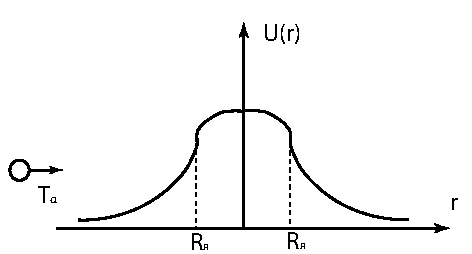
\includegraphics{4_2.pdf}
    \end{tabular}
\end{table}
        \[
            T_\alpha \leq U_{max} \approx \frac{3}{2}\frac{q_1 q_2}{r_{min}},
        \]
    где \( q_1 = 2e \) -- заряд \( \alpha \)-частицы, \( q_2 = 82e \) -- заряд
    ядра свинца.
    
    Из формулы получим: \( r_{min} \approx R_\emph{я} \approx 9,6\cdot10^{-10} \)~см.
    
    Для более точного расчёта \( T = \cfrac{2ze^2}{r_{min}} \), где z = 82.\\

\newpage

% 4.3 --------------
\item \( \alpha \)-частица с кинетической энергией \( T \) налетает с прицельным
параметром \( 0,\!9\cdot10^{-11} \)~см на покоящееся ядро свинца. Найти:
\begin{enumerate}
    \item модуль приращения вектора импульса рассеянной \( \alpha \)-частицы,
    если \( T = 2,\!3 \)~МэВ;
    \item при каком значении \( T \) модуль приращения вектора импульса
    рассеяния \( \alpha \)-частицы будет максимальным для данного прицельного
    параметра. Каков при этом угол рассеяния?
\end{enumerate}

\emph{Решение:}

\newpage

% 4.4 --------------
\item Нерелятивистская частица массой \( m \) и кинетической энергией \( T \)
испытала упругое рассеяние на первоначально покоящемся ядре с массой \( M \).
Найти в Ц-системе импульс каждой частицы и их суммарную энергию.

\emph{Решение:}

\begin{align*}
    p = \mu v_\emph{отн} = \frac{m_2}{m1+m2}\cdot p_1, & \quad p_1 = \sqrt{2mT}. \\
    \mu = \frac{m1\cdot m2}{m1+m2}, \quad m1 & = m, \quad m_2 = M; \\
    p = \frac{\sqrt{2mT}}{1+\frac{m}{M}}; \quad
    E = & \frac{p^2}{2\mu} = \frac{T}{1+\frac{m}{M}}.
\end{align*}

\newpage

% 4.5 --------------
\item Найти максимальное значение угла рассеяния \( \alpha \)-частицы на
первоначально покоящемся дейтроне.

\emph{Решение:}

\newpage

% 4.6 --------------
\item В результате упругого рассеяния протона с кинетической энергией
\( T = 13,\!0 \)~кэВ в кулоновском поле покоящегося ядра \( ^4\mathrm{He} \)
последнее испытало отдачу под углом \( \theta = 60^\circ \) к направлению
движения налетающего протона. Вычислить прицельный параметр.

\emph{Решение:}

    Прицельный параметр \( b \) можно найти, воспользовавшись формулой:
    \[
        \tg\frac{\theta}{2} = \frac{q_1 q_2}{2bT_1},
    \]
    откуда
    \[
        b = \frac{q_1 q_2}{2T_1}\ctg\frac{\theta}{2}.
    \]
    
    Так как \( \theta \) и \( T \) -- это параметры в Ц-системе, необходимо
    перейти в Л-систему:
    \[
        T_1 = \frac{m_2}{m_1 + m_2} = \frac{4}{5}T.
    \]
    Следовательно
    \[ 
        b = \frac{2e^2\cdot 5}{2\cdot 4\cdot T}\ctg{30^\circ} \approx
        2,\!4\cdot 10^{-11} \text{ см} 
    \]

\newpage

% 4.7 --------------
\item \( \alpha \)-частица с кинетической энергией \( T = 5,\!0 \)~кэВ упруго
рассеялась в кулоновском поле покоящегося дейтрона. Найти прицельный
параметр, соответствующий максимально возможному углу рассеяния
\( \alpha \)~частицы в Л-системе.

\emph{Решение:}

\end{enumerate}